% debut d'un fichier latex standard
\documentclass[a4paper,12pt,oneside]{article}
\usepackage[top=3cm, bottom=3.5cm]{geometry}
% pour l'inclusion de figures en eps,pdf,jpg,....
\usepackage{graphicx}
\usepackage{wrapfig}
\usepackage{subcaption}
% quelques symboles mathematiques en plus
\usepackage{amsmath}
% le tout en langue francaise
\usepackage[french]{babel}
\usepackage[T1]{fontenc}
% on peut ecrire directement les characteres avec l'accent
% a utiliser sur Linux/Windows
\usepackage[utf8]{inputenc}
\usepackage[rightcaption
]{sidecap}
\usepackage[export]{adjustbox}
% a utiliser sur le Mac
%\usepackage[applemac]{inputenc}
% pour l'inclusion de links dans le document (pdflatex)
\usepackage[colorlinks,bookmarks=false,linkcolor=blue,urlcolor=blue]{hyperref}
%
\usepackage{caption}
\usepackage{float}
% quelques abreviations utiles
\def \be {\begin{equation}}
\def \ee {\end{equation}}
\def \bf {\begin{figure}}
\def \ef {\end{figure}}
\def \dd  {{\rm d}}
\def \t {\theta}
\def \vt {\Dot{\theta}}

\newcommand{\norme}[1]{\left\Vert #1 \right\Vert}
%
\newcommand{\mail}[1]{{\href{mailto:#1}{#1}}}
\newcommand{\ftplink}[1]{{\href{ftp://#1}{#1}}}












%%%%%%%%%%%%%%%%%%%%%%%%%%%%%%%%%%%%%%%%%%%%%%%%%%%%%%%%%%%%%%%%%%%%%%%%%%%%%%%%%%%%%%%%%%%%%%%%%%%%%%%%
%%%%%%%%%%%%%%%%%%%%%%%%%%%%%%%%%% le document commence ici %%%%%%%%%%%%%%%%%%%%%%%%%%%%%%%%%%%%%%%%%%%%
%%%%%%%%%%%%%%%%%%%%%%%%%%%%%%%%%%%%%%%%%%%%%%%%%%%%%%%%%%%%%%%%%%%%%%%%%%%%%%%%%%%%%%%%%%%%%%%%%%%%%%%%
\begin{document}
% le titre et l'auteur
\title{Physique numérique I : exercice 3}
\date{\today}
\author{Victor Despland, Timothée Dao\\{\small \mail{victor.despland@epfl.ch}, \mail{timothee.dao@epfl.ch}}}
\maketitle
\tableofcontents



%%%%%%%%%%%%%%%%%%%%%%%%%%%%%%%%%%%%%%%%%%%%%%%%%%%%%%%%%%%%%%%%%%%%%%%%%%%%%%%%%%%%%%%%%%%%%%%%%%%%%%%%
%%%%%%%%%%%%%%%%%%%%%%%%%%%%%%%%%%%%%%%%%%%%%%%%%%%%%%%%%%%%%%%%%%%%%%%%%%%%%%%%%%%%%%%%%%%%%%%%%%%%%%%%
%%%%%%%%%%%%%%%%%%%%%%%%%%%%%%%%%%%%%%%%%%%%%%%%%%%%%%%%%%%%%%%%%%%%%%%%%%%%%%%%%%%%%%%%%%%%%%%%%%%%%%%%
\newpage
\newpage \section{Introduction}

\intextsep=-0.5cm
\begin{wrapfigure}{r}{0.4\textwidth}
    \centering
    \includegraphics[width=0.33\textwidth]{schemaDonnee}
    \caption{\cite{donneeEX2}}
\end{wrapfigure}


Le but de cet exercice est d'étudier le mouvement d'un pendule, composé d'un point matériel P de masse $m=0.1\rm kg$ et d'une tige rigide de masse négligeable et de longueur $L=0.1\rm m$. Ce pendule est attaché à un point $O'$ fixée dans une boîte. La boîte effectue un mouvement oscillatoire verticale $y_{O'}(t) = d \sin(\Omega t)$, avec une amplitude $d$ et une fréquence $\Omega$ données. Les frottements exercent une force $\mathbf{F}_{frot}=-\kappa \mathbf{v}_P)_\mathcal{R'}$, où $\kappa$ est un coefficient de frottement donné et $\textbf{v}_P)_\mathcal{R'}$ est la vitesse de P dans le référentiel $\mathcal{R'}$ de la boîte. On prendra pour tout l'exercice $g=9.81 \rm ms^{-2}$.

Les notions de sections de Poincaré, de chaos et d'attracteurs (étranges) seront abordées.

\intextsep=0.5cm



%%%%%%%%%%%%%%%%%%%%%%%%%%%%%%%%%%%%%%%%%%%%%%%%%%%%%%%%%%%%%%%%%%%%%%%%%%%%%%%%%%%%%%%%%%%%%%%%%%%%%%%%
%%%%%%%%%%%%%%%%%%%%%%%%%%%%%%%%%%%%%%%%%%%%%%%%%%%%%%%%%%%%%%%%%%%%%%%%%%%%%%%%%%%%%%%%%%%%%%%%%%%%%%%%
%%%%%%%%%%%%%%%%%%%%%%%%%%%%%%%%%%%%%%%%%%%%%%%%%%%%%%%%%%%%%%%%%%%%%%%%%%%%%%%%%%%%%%%%%%%%%%%%%%%%%%%%
\section{Calculs analytiques}


%%%%%%%%%%%%%%%%%%%%%%%%%%%%%%%%%%%%%%%%%%%%%%%%%%%%%%%%%%%%%%%%%%%%%%%%%%%%%%%%%%%%%%%%%%%%%%%%%%%%%%%%
\subsection{Équations différentielles du mouvement}

On choisit un système de coordonnées polaires dans le référentiel de la boîte. La position, la vitesse et l'accélération sont donc respectivement données par 
\setlength\arraycolsep{0pt}
\[
\begin{array}{r @{{}={}} l}
\mathbf{p} & \rho \mathbf{e_r} \\
\mathbf{v} & \Dot{\rho} \mathbf{e_r} + \rho\vt \mathbf{e_\t} \\
\mathbf{a} & (\Ddot{\rho} - \rho \vt^2) \mathbf{e_r} + (\rho \Ddot{\t} + 2 \Dot{\rho} \vt) \mathbf{e_\t}
\end{array}
\]
La condition de la tige rigide implique $\rho = L = const$ et donc $\Dot{\rho}=0$, réduisant ainsi les expressions précédentes à 
\[
\begin{array}{r @{{}={}} l}
\mathbf{p} & L \mathbf{e_r} \\
\mathbf{v} & L\vt \mathbf{e_\t} \\
\mathbf{a} & - L \vt^2 \mathbf{e_r} + L \Ddot{\t} \mathbf{e_\t}
\end{array}
\]

Les forces en présence sont :
\[
\begin{array}{l @{{}={}} l}
\mathbf{F}_p & - mg \cos{\t} \mathbf{e_r} - mg \sin{\t} \mathbf{e_\t} \\
\mathbf{F}_{frot} & -\kappa L \vt \mathbf{e_\t} \\
\mathbf{T}_{tige} & -T \mathbf{e_r} \\
\mathbf{F}_{inertie} & m d \Omega^2 \sin{(\Omega t)}\cos{(\t)} \mathbf{e_r} - m d \Omega^2 \sin{(\Omega t)}\sin{(\t)} \mathbf{e_\t}
\end{array}
\]

De la 2ème loi de Newton, $\sum \textbf{F}=m\textbf{a}$ et projetant sur l'axe $\t$ on obtient :
\be
mL \Ddot{\t} = - mg \sin{\t} - \kappa L \vt - m d \Omega^2 \sin{(\Omega t)}\sin{(\t)}
\ee

On en tire donc le système d'équations différentielles (non-linéaires) caractérisant notre problème :
\be
\frac{\dd }{\dd t} 
\left( \begin{array}{c} \t \\ \vt  \end{array} \right)
=
\left( \begin{array}{c}
   \vt \\
   -[g+d\Omega^2\sin{(\Omega t)}]\sin{(\t)}/L - \kappa\vt/m
\end{array} \right)
\label{eq1}
\ee


%%%%%%%%%%%%%%%%%%%%%%%%%%%%%%%%%%%%%%%%%%%%%%%%%%%%%%%%%%%%%%%%%%%%%%%%%%%%%%%%%%%%%%%%%%%%%%%%%%%%%%%%
\subsection{Puissance, travail et énergie} 
Dans le problème qui nous intéresse, la seule force dérivant d'un potentiel est la force de pesanteur. En prenant comme point de référence (pour l'énergie potentiel de gravitation) $h=0$ à $y'=-L$, l'expression de l'énergie mécanique se résume à :
\be
E_{mec}=E_{pot}+E_{cin}=mgh+\frac{1}{2}m\norme{\mathbf{v}}^2=mgL(1-\cos{\t})+\frac{1}{2}m(L \vt)^2
\ee

Deux forces non-conservatives travaillent : la force de frottement et la force d'inertie. L'expression de leur puissance est donnée par 
\be 
\begin{array}{r @{{}={}} l}  
P_{\rm NC} & \langle \mathbf{F}_{\rm NC} , \mathbf{v} \rangle \\
& \langle md\Omega^2\sin{(\Omega t)}\cos{(\t)}\mathbf{e_r}-(\kappa L \vt +  md\Omega^2\sin{(\Omega t)}\sin{(\t)})\mathbf{e_\t},L \vt \mathbf{e_\t} \rangle \\
& -(\kappa L \vt +  md\Omega^2\sin{(\Omega t)}\sin{(\t)})L \vt
\end{array}
\ee
Le travail $W_{\rm NC}$ des forces non conservatives entre $t_0$ et $t$ est alors donné par 
\be
W_{\rm NC} = \int_{t_0}^{t}P_{\rm NC} dt
\ee



%%%%%%%%%%%%%%%%%%%%%%%%%%%%%%%%%%%%%%%%%%%%%%%%%%%%%%%%%%%%%%%%%%%%%%%%%%%%%%%%%%%%%%%%%%%%%%%%%%%%%%%%
\subsection{Résolution du système dans le cas $d=0$, $\kappa=0$ et $\t \ll 1$ \label{resolutionEqt}} 
On étudie ici le cas où il n'y a ni excitation extérieure ($d=0$), ni amortissement ($\kappa =0$). De plus, on suppose que le pendule effectue uniquement des petits mouvements, c'est-à-dire $\t \ll 1$ et donc $\sin{(\t)} \approx \t$. Dans ce cas là, on peut résoudre les équations du mouvement pour le pendule.
L'Eq.\eqref{eq1} se réduit alors à au système d'équations différentielles suivant :
\be
\frac{\dd }{\dd t} 
\left( \begin{array}{c} \t \\ \vt  \end{array} \right)
=
\left( \begin{array}{c}
   \vt \\
   -\omega_0^2\theta
\end{array} \right)
\label{eq4}
\ee
où $\omega_0=\sqrt{g/L}$ dénote la fréquence propre du système.
La solution générale est alors donnée par:
\be
\theta(t)=A\cos{(\omega_0t+\phi)}
\label{eq:SolutionGenerale}
\ee


On notera l'angle et la vitesse angulaire, donnés par la solution analytique, au temps $t=t_i$ par $\t(t_i)$ et $\vt(t_i)$, avec $t_i=i \times \Delta t$ et $i=0,1,2,...$.



%%%%%%%%%%%%%%%%%%%%%%%%%%%%%%%%%%%%%%%%%%%%%%%%%%%%%%%%%%%%%%%%%%%%%%%%%%%%%%%%%%%%%%%%%%%%%%%%%%%%%%%%
%%%%%%%%%%%%%%%%%%%%%%%%%%%%%%%%%%%%%%%%%%%%%%%%%%%%%%%%%%%%%%%%%%%%%%%%%%%%%%%%%%%%%%%%%%%%%%%%%%%%%%%%
%%%%%%%%%%%%%%%%%%%%%%%%%%%%%%%%%%%%%%%%%%%%%%%%%%%%%%%%%%%%%%%%%%%%%%%%%%%%%%%%%%%%%%%%%%%%%%%%%%%%%%%%
\newpage \section{Méthodes numériques}
Le système d'équations différentielles définissant ce problème est
\be \label{sysDef}
\mathbf{y}  
=  \left( \begin{array}{c} \t \\ \vt \end{array} \right), \quad 
\mathbf{f}(\mathbf{y},t)  
=  \frac{\dd \mathbf{y}}{\dd t}  
=  \frac{\dd }{\dd t}\left( \begin{array}{c} \t \\ \vt \end{array} \right) 
=  \left( \begin{array}{c} \vt \\ a_\t  \end{array} \right)
\ee
où $a_\t=a_\t(\t,\vt,t)$ est explicitée dans l'Eq.\eqref{eq1}.
On notera $\t_i$ et $\vt_i$ les approximations (obtenues numériquement) de $\t(t_i)$ et $\vt(t_i)$ respectivement, avec $t_i=i \times \Delta t$ et $i=0,1,2,...$. 


%%%%%%%%%%%%%%%%%%%%%%%%%%%%%%%%%%%%%%%%%%%%%%%%%%%%%%%%%%%%%%%%%%%%%%%%%%%%%%%%%%%%%%%%%%%%%%%%%%%%%%%%
\subsection{Schéma de Verlet \cite{notesDeCours}}
On utilisera le schéma de Verlet, qui dans notre cas de figure est donné par :
\be
\left\{ \begin{array}{r @{{}={}} l} 
\t_{i+1} & \t_{i} 
             + \vt_{i} \Delta t 
             + \frac{1}{2}a(\t_{i},\vt_{i},t_{i}) (\Delta t)^2\\
\vt_{i+1/2} & \vt_{i}
                 + \frac{1}{2}a(\t_{i},\vt_{i},t_{i}) \Delta t \\
\vt_{i+1} & \vt_{i} 
               + \frac{1}{2}[a(\t_{i},\vt_{i+1/2},t_{i})+a(\t_{i+1},\vt_{i+1/2},t_{i+1})] \Delta t
\end{array} \right.
\ee
On peut montrer que le schéma est stable si $\omega_0 \Delta t \leq 2$.



%%%%%%%%%%%%%%%%%%%%%%%%%%%%%%%%%%%%%%%%%%%%%%%%%%%%%%%%%%%%%%%%%%%%%%%%%%%%%%%%%%%%%%%%%%%%%%%%%%%%%%%%
%%%%%%%%%%%%%%%%%%%%%%%%%%%%%%%%%%%%%%%%%%%%%%%%%%%%%%%%%%%%%%%%%%%%%%%%%%%%%%%%%%%%%%%%%%%%%%%%%%%%%%%%
%%%%%%%%%%%%%%%%%%%%%%%%%%%%%%%%%%%%%%%%%%%%%%%%%%%%%%%%%%%%%%%%%%%%%%%%%%%%%%%%%%%%%%%%%%%%%%%%%%%%%%%%
\newpage \section{Résultats numériques}


%%%%%%%%%%%%%%%%%%%%%%%%%%%%%%%%%%%%%%%%%%%%%%%%%%%%%%%%%%%%%%%%%%%%%%%%%%%%%%%%%%%%%%%%%%%%%%%%%%%%%%%%
\subsection{Petits mouvements sans excitation ni amortissement}
Cette première série de simulations consiste à étudier le cas de petits mouvements sans excitation ni amortissement comme décrit à la section \ref{resolutionEqt}. On prendra comme temps final $t_{fin}=20 \rm s$ et comme conditions initiales $\t_0=10^{-6} \rm{rad}$ et $\vt=0$.

\paragraph{Comparaison des solutions numériques et analytiques} %%%%%%%%%%%%%%%%%%%%%%%%%%%%%%%%%%%%
La solution analytique générale est donnée par l'Eq.\ref{eq:SolutionGenerale} et les conditions initiales sont $\theta(0)=\theta_0$ et $\vt=0$. On obtient ainsi $\phi=0$ et $A=\theta_0$ et donc
\be
 \left(\begin{array}{c} \t (t) \\ \vt (t) \end{array} \right) =
\left(\begin{array}{c} \t_0\cos{(\omega_0 t)} \\ -\omega_0\t_0 \sin{(\omega_0 t)} \end{array} \right)
\ee
\begin{figure}[H]
    \begin{subfigure}[b]{0.5\textwidth}
    \centering
    \includegraphics[scale=0.4]{thetaT.eps}
    \caption{$\theta$ en fonction de t}
    \label{fig:ThetaT}
\end{subfigure}
\begin{subfigure}[b]{0.5\textwidth}
    \includegraphics[scale=0.4]{ThetadotT.eps}
    \caption{$\dot{\theta} $ en fonction de t}
    \label{fig:ÎhetadotTl}
\end{subfigure}
\ContinuedFloat
    \begin{subfigure}[b]{1\textwidth}
    \centering
    \includegraphics[scale=0.4]{ThetaThetadot.eps}
    \caption{$\dot{\theta}$ en fonction de $\theta$}
    \label{fig:ThetaThetadot}
\end{subfigure}
\caption{Simulations réalisées avec la méthode de Verlet pour un pendule simple. Les solutions analytique et numérique pour $\Delta t=0.008\rm{s}$ sont confondus à l'échelle étudiée.}
\label{fig:SimulationsPremierPoint}
\end{figure}
On réalise des simulations pour trois $\Delta t$ différents. Ce sont à chaque fois des cas stables, c'est-à-dire où $\omega_0 \Delta t \leq 2$. Dans le cas où $\Delta t=0.2\rm{s}$ (en vert sur la Fig.\ref{fig:SimulationsPremierPoint}), on a $\omega \Delta t = 1.98$ et on est donc proche de l'instabilité. On constate également que des battements se forme sur les Fig.\ref{fig:ThetaT} et Fig.\ref{fig:ÎhetadotTl}.
Dans le cas où $\Delta t=0.008\rm{s}$ (en cyan sur la Fig.\ref{fig:SimulationsPremierPoint}), la solution numérique est confondue avec la solution analytique.


\paragraph{Étude de convergence} %%%%%%%%%%%%%%%%%%%%%%%%%%%%%%%%%%%%%%%%%%%%%%%%%%%%%%%%%%%%%%%%%%%
On réalise une série de simulations en faisant varier le pas de temps $\Delta t$ entre $10^{-2} \rm s$ et $10^{-5} \rm s$. Pour chaque simulation, on calcule l'erreur sur l'angle $\t$ au temps $t=t_{fin}$.
\begin{figure}[H]
    \centerline{\includegraphics[width=0.95\linewidth,angle=0]{etudeConvDt1}}
\caption{ \label{etudeConvDt1}\em
Étude de convergence en $\Delta t$ pour un pendule simple. 
}
\end{figure}
Les résultats sont présentés sur la Fig.\ref{etudeConvDt1} et on peut donc confirmer que l'ordre de la méthode de Verlet est de 2, en constatant que la pente du graphe est égale à deux.

\paragraph{Conservation de l'énergie} %%%%%%%%%%%%%%%%%%%%%%%%%%%%%%%%%%%%%%%%%%%%%%%%%%%%%%%%%%%%%%
Dans ce cas de figure, seulement la force de pesanteur entre en jeu dans le bilan d'énergie (la tension de la tige ne travaille pas). L'énergie mécanique est donc censée être conservée :
\be
E_{mec}=mgL(1-\cos{\t})+ \frac{1}{2}m(L\vt)^2= const
\ee
On peut vérifier cela numériquement (Fig.\ref{energy1}). On remarque que l'énergie n'est pas exactement conservée mais elle est bornée et conservée en moyenne (cependant la moyenne est légèrement inférieure à la valeur théorique). Pour $\Delta t=0.008 \rm{s}$, l'énergie est quasiment confondu avec l'énergie théorique à l'échelle étudiée. En conclusion, le schéma de Verlet est bien symplectique dans le cas d'un oscillateur harmonique.
\begin{figure}[H]
    \centerline{\includegraphics[width=0.95\linewidth,angle=0]{EnergyT.eps}}
\caption{ \label{energy1}\em
Énergie mécanique en fonction du temps pour trois simulations numériques et la solution analytique.
}
\end{figure}

%%%%%%%%%%%%%%%%%%%%%%%%%%%%%%%%%%%%%%%%%%%%%%%%%%%%%%%%%%%%%%%%%%%%%%%%%%%%%%%%%%%%%%%%%%%%%%%%%%%%%%%%
\subsection{Grands mouvement sans excitation ni amortissement \label{grandMvmt}}
On s'intéresse ici au cas de grands mouvements sans excitation ni amortissement ($d=0$ et $\kappa=0$). On prendra comme temps final $t_{fin}=20 \rm s$ et comme conditions initiales $\t_0 \in \mathopen{]}0\,;\pi \mathopen{[}$ et $\vt=0$.

On veut montrer que la période du pendule dépend de l'angle initial $\t_0$ pour des grands mouvements. \\
On peut montrer analytiquement qu'on a $T(\t_0)=\frac{4}{\omega_0}K(\sin{(\t_0/2)})$, avec $K(k)=\int_{0}^{\pi/2}(1-k^2\sin^2\t)^{-1/2}\dd \t$. \\
Pour trouver la période numériquement, on constate que le temps entre deux changements de signe de $\t$ correspond à une demi période. En notant $t_a$ et $t_b$ les instants du premier et respectivement deuxième changement de signe, on a donc $T/2=t_b-t_a$. Cependant, dans le cas de simulations numériques, on ne connaît en général que les instants $t_{a,1}$ et $t_{a,2}=t_{a,1}+\Delta t$, les instants respectivement juste avant et juste après le changement de signe. On peut choisir arbitrairement $t_{a,1}$ ou $t_{a,2}$, ainsi l'instant $t_a$ du premier changement de signe n'est connu qu'avec une incertitude de $\Delta t$. En faisant la moyenne des instants $t_{a,1}$ et $t_{a,2}$, on réduit l'incertitude à $\Delta t /2$. On peut encore améliorer ce résultat en approximant $\t(t)$ par une droite entre $t_{a,1}$ et $t_{a,2}$ :
\be
t_a \approx t_{a,1} + \frac{t_{a,2}-t_{a,1}}{ \t_{a,1}-\t_{a,2}} \t_{a,1}
\ee
où $\t_{a,1}$, resp. $\t_{a,2}$, dénote $\t$ (obtenu numériquement) à l'instant $t_{a,1}$, resp. $t_{a,2}$. 

Ainsi, en calculant également $t_c$, l'instant du troisième changement de signe, on obtient finalement une expression pour la période :
\be 
T_{num}=t_c-t_a \approx  t_{c,1} - t_{a,1} + \frac{t_{c,2}-t_{c,1}}{\t_{c,1}-\t_{c,2}} \t_{c,1} - \frac{t_{a,2}-t_{a,1}}{\t_{a,1}-\t_{a,2}} \t_{a,1}
\ee 

Les résultats sont présentés sur la Fig.\ref{theta0}. On peut constater que les les solutions analytique et numérique concordent. L'erreur sur la période, $\lvert T(\t_0)-T_{num}(\t_0) \rvert$, est approximativement 7 ordres de grandeur plus petit que la période obtenue numériquement (Fig.\ref{theta0error}), ce qui donne une erreur relative très faible.
\begin{figure}[H]
    \centerline{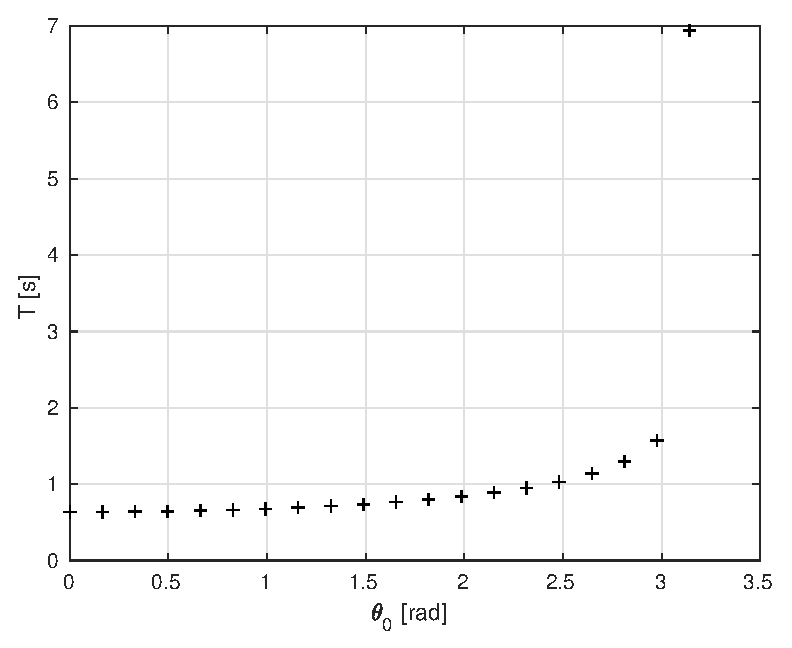
\includegraphics[width=0.95\linewidth,angle=0]{theta0}}
\caption{ \label{theta0}\em
Période du pendule en fonction de l'angle d'oscillation maximum, obtenue par la théorie analytique et par des simulations numériques.
}
\end{figure}


\begin{figure}[H]
    \centerline{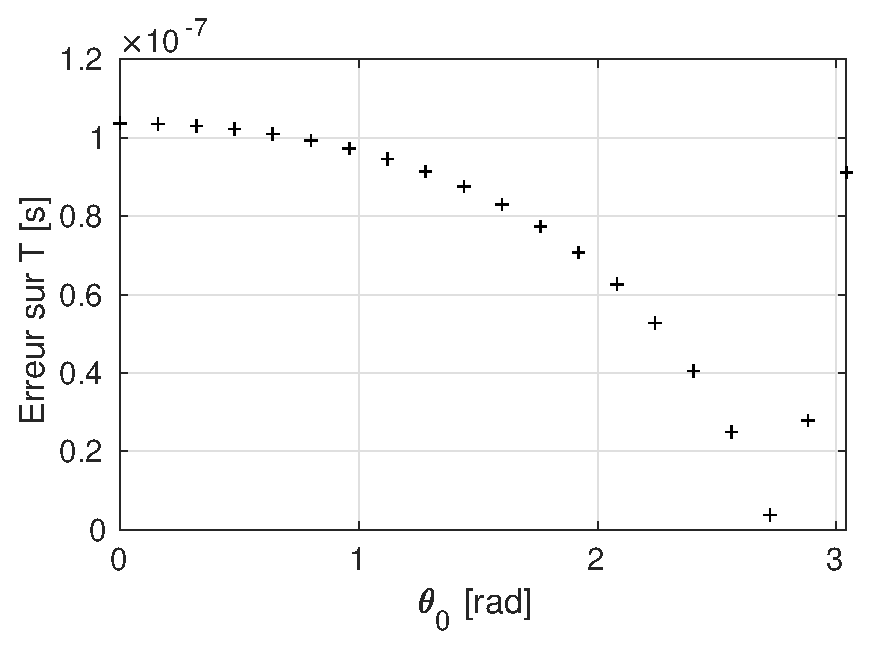
\includegraphics[width=0.95\linewidth,angle=0]{theta0error}}
\caption{ \label{theta0error}\em
Erreur sur la période avec $\Delta t=0.0002\rm{s}$.
}
\end{figure}


%%%%%%%%%%%%%%%%%%%%%%%%%%%%%%%%%%%%%%%%%%%%%%%%%%%%%%%%%%%%%%%%%%%%%%%%%%%%%%%%%%%%%%%%%%%%%%%%%%%%%%%%
\subsection{Excitation résonnante}
On étudie dans cette section le cas d'oscillations sans amortissement ($\kappa =0$), mais avec une excitation extérieure ($d=0.03\rm{m}$). La fréquence d'oscillation de la boîte est égale à la fréquence propre du pendule ($\Omega=\omega_0$) et les conditions initiales sont $\t_0=0$, $\vt_0=10^{-2} \rm{rad/s}$. On prendra $t_{fin}=250\rm{s}$.

Nous allons dans un premier temps vérifier numériquement le théorème de l'énergie mécanique :
\be
E_{mec}(t)=E_{mec}(t_0)+\int_{t_0}^{t}P_{\rm NC}dt
\ee
La méthode d'intégration numérique du trapèze sera utilisée pour approcher le travail des force non conservatives entre $t_0=0$ et $t_n=n \Delta t$ :
\be
W_{\rm NC}=\int_{t_0}^{t_n}P_{\rm NC}(t)dt \approx \sum_{i=0}^{n-1}\frac{P_{\rm NC}(t_{i+1})-P_{\rm NC}(t_{i})}{2}\Delta t
\ee

Les résultats des simulations sont présentés sur la Fig.\ref{energyW}, avec un agrandissment sur la Fig.\ref{energyWZoom}. Le théorème de l'énergie mécanique est bien vérifié comme la différence entre l'énergie mécanique et le travail des forces non conservatives à un instant donné, qui est bornée, quasiment constante et égale à l'énergie mécanique initiale : $E_{mec}(t_n)-W_{\rm{NC}}=E_{mec}(t_0)$.
\begin{figure}[H]
    \centerline{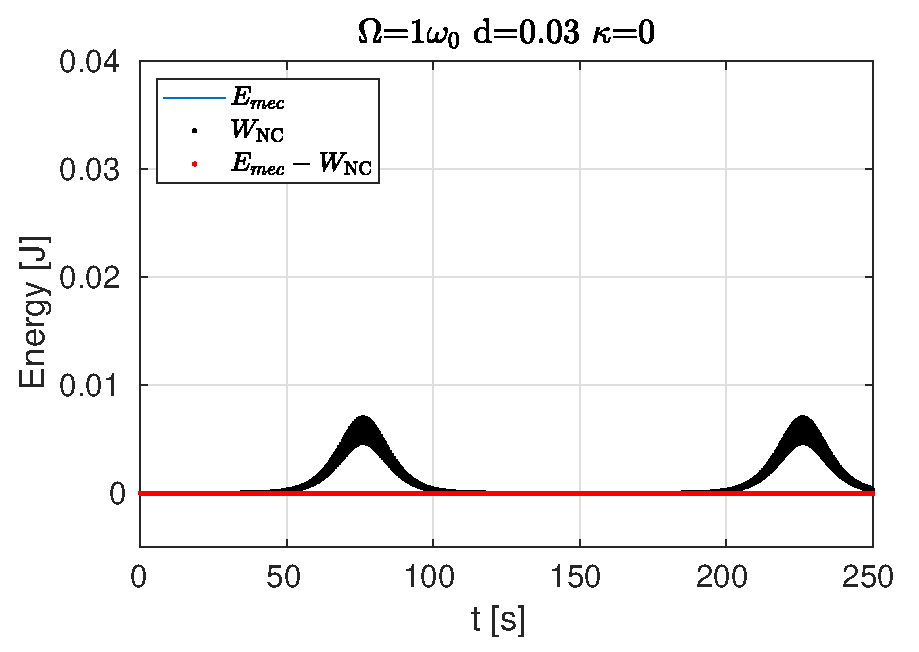
\includegraphics[width=0.93\linewidth,angle=0]{energyW}}
\caption{ \label{energyW}\em
Travail des force non-conservatives et énergie mécanique en fonction du temps pour un pendule excité mais non-amorti.
}
\end{figure}
\begin{figure}[H]
    \centerline{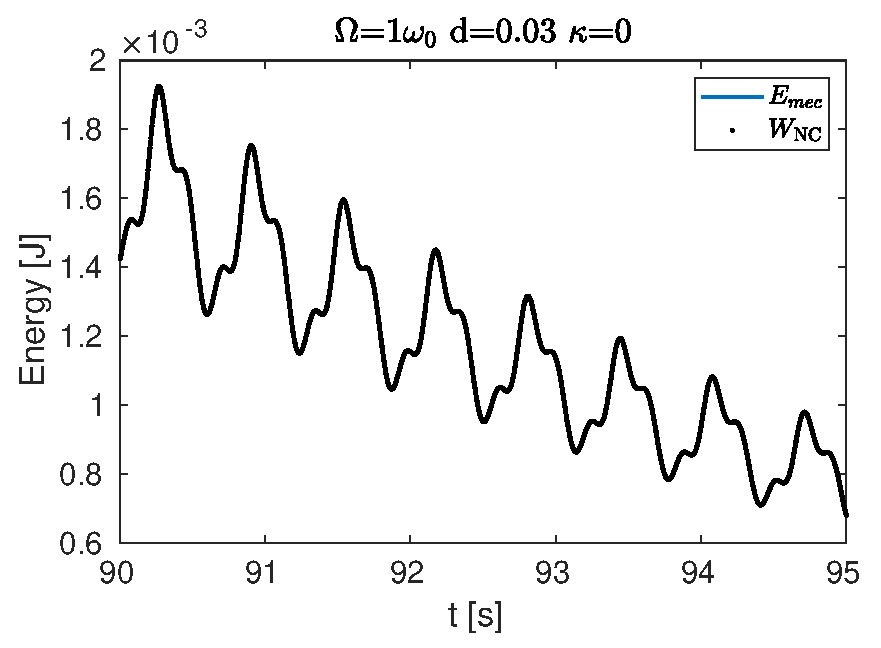
\includegraphics[width=0.93\linewidth,angle=0]{energyWZoom}}
\caption{ \label{energyWZoom}\em
Agrandissement de la Fig.\ref{energyW}.
}
\end{figure}

On peut maintenant faire varier $\Omega$ autour de $\omega_0$ et étudier le comportement du pendule, et notamment le maximum de l'énergie mécanique : $\max_{t}(E_{mec}(t))$. Comme on peut le voir sur la Fig.\ref{rechercheOmega}, où le maximum de l'énergie est représenté en fonction de $\Omega$, l'énergie maximum augmente brutalement peu avant $\Omega=\omega_0$, puis diminue quasiment linéairement pour atteindre à nouveau des valeurs d'énergie maximum relativement faibles. De la théorie analytique, l'énergie d'un oscillateur harmonique est censé exploser lorsque la fréquence d'excitation est égale à la fréquence propre du système. Cependant, dans notre cas de figure, dès que l'énergie augmente, le pendule va effectuer des oscillations de plus grandes amplitudes, au point où on ne peut plus le considérer comme un oscillateur harmonique. En fait, comme on l'a montré dans le section \ref{grandMvmt}, la période dépend de l'amplitude et ainsi l'énergie maximum n'est pas atteinte lorsque $\Omega=\omega_0$ mais légèrement avant. Ceci pour la raison précise que lors de grands mouvements, la pulsation du pendule n'est plus $\omega_0$, mais plus petite (la période augmente avec l'amplitude).
\begin{figure}[H]
    \centerline{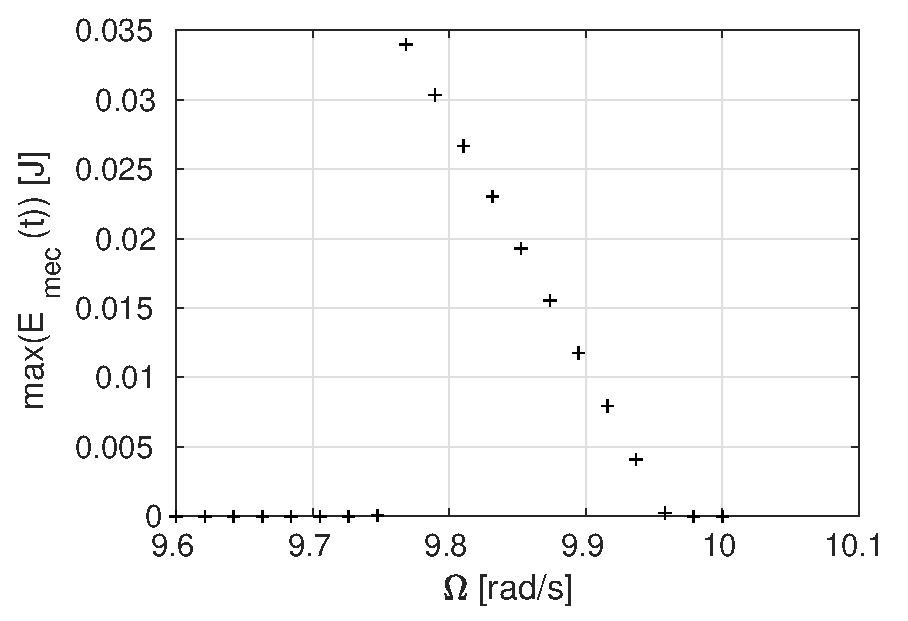
\includegraphics[width=0.95\linewidth,angle=0]{rechercheOmega}}
\caption{ \label{rechercheOmega}\em
Maximum de l'énergie mécanique en fonction de la fréquence d'excitation $\Omega$, aux alentours de $\omega_0$
}
\end{figure}
\label{sec:reso}


%%%%%%%%%%%%%%%%%%%%%%%%%%%%%%%%%%%%%%%%%%%%%%%%%%%%%%%%%%%%%%%%%%%%%%%%%%%%%%%%%%%%%%%%%%%%%%%%%%%%%%%%
\subsection{Excitation paramétrique}
Dans cette section, on étudie des oscillations avec amortissement ($\kappa=0.05\rm{kgs^{-2}}$) et avec une excitation extérieure ($d=0.005\rm{m}$). Cette fois-ci la pulsation de l'excitation est égale à deux fois la pulsation propre du système ($\Omega=2\omega_0$). On prendra comme conditions initiales $\theta_0=0, \dot{\theta_0}=10^{-2}\rm{rad/s}$ et $t_{fin}=100\rm{s}$. \\
On constate sur la Fig.\ref{fig:energy2W} que le théorème de l'énergie mécanique est bel et bien conservée (ligne rouge). Jusqu'à 25s, l'énergie est stable et elle augmente ensuite de manière brutale jusqu'à atteindre un maximum pour diminuer ensuite et se stabiliser. Comme à la section \ref{sec:reso}, lorsque l'amplitude du pendule augmente sa pulsation diminue jusqu'à atteindre un point où l'oscillation s'est suffisamment décalé par rapport à l'excitation pour que les deux ne soient plus en phase de manière constructive. Cependant, comme on considère l'action des frottements, ils seront à ce moment là suffisamment élevée pour ralentir le pendule et ainsi permettre au pendule de presque se stabiliser à $\t \neq 0$, il effectue en fait des petites oscillations autour de cet angle.

\begin{figure}[H]
    \centering
    \includegraphics[width=0.95\linewidth]{energyW2.eps}
    \caption{Travail des force non-conservatives et énergie mécanique en fonction du temps pour un pendule excité et amorti.}
    \label{fig:energy2W}
\end{figure}

Sur la Fig.\ref{fig:recherche2omega}, lorsque l'on fait varier $\Omega$ au voisinage de $2\omega_0$ le maximum de l'énergie se comporte de la même manière que dans le cas précédent (section \ref{sec:reso}, Fig.\eqref{rechercheOmega}). Le maximum de l'énergie est faible jusqu'à $\Omega \simeq 19\rm{rad/s}$, pour ensuite monter abruptement au maximum lorsque $\Omega \simeq 19.25\rm{rad/s}$ puis redescendre linéairement jusqu'à $\Omega \simeq 20.75\rm{rad/s}$ et redevenir faible ensuite. Le fait que le maximum se situe avant le double de la pulsation propre $\omega_0$ est de nouveau causé par la diminution de la pulsation lorsque $\t $ est grand, donc $2\omega_0$ ne correspond pas exactement au double de la pulsation. 
\begin{figure}[H]
    \centering
    \includegraphics[width=0.95\linewidth]{energyW2Zoom.eps}
    \caption{Agrandissment de la Fig.\ref{fig:energy2W}.}
    \label{fig:energyW2zoom}
\end{figure}
\begin{figure}[H]
    \centering
    \includegraphics[scale=0.6]{recherche2Omega.eps}
    \caption{Maximum de l'énergie de simulations au voisinage du double de la fréquence propre du système.}
    \label{fig:recherche2omega}
\end{figure}
%%%%%%%%%%%%%%%%%%%%%%%%%%%%%%%%%%%%%%%%%%%%%%%%%%%%%%%%%%%%%%%%%%%%%%%%%%%%%%%%%%%%%%%%%%%%%%%%%%%%%%%%
\subsection{Section de Poincaré, non amorti}
\paragraph{Étude de convergence}
Nous étudions ici le cas d'un pendule excité ($d \neq 0$), mais non amorti ($\kappa=0$). Nous réalisons dans un premier temps une étude de convergence en $\Delta t$ pour vérifier que la méthode numérique converge bien dans le cas d'un pendule excité. Les résultats sont présentés sur la Fig.\ref{etudeConvDt2}. On peut constater qu'en représentant l'angle $\t$ final en fonction de $(\Delta t)^2$, les points s'alignent pour former une droite, confirmant ainsi que la méthode converge à l'ordre 2.
\begin{figure}[H]
    \centerline{\includegraphics[width=0.95\linewidth,angle=0]{etudeConvDt2}}
\caption{ \label{etudeConvDt2}\em
Étude de convergence en $\Delta t$ pour un pendule excité mais non-amorti.
}
\end{figure}
\paragraph{Sections de Poincaré}
Nous réalisons ensuite des projections de l'espace $(t,\t,\vt)$. Pour réaliser ces projections, nous prendrons l'espace des phases ($\t,\vt$) uniquement aux temps qui sont des multiples de la période d'excitation $\Omega$. Les sections de Poincaré que nous allons étudier sont donc données par $\{(\t(t_i),\vt(t_i)) : t_i=i2\pi/\Omega \}_{i \in [i_s,i_e]}$, en prenant typiquement $i_s\approx 100$ et $i_e \approx 10000$. 

On peut voir sur les Fig.\ref{poincare1} et Fig.\ref{poincare2} que chaque condition initiale donne une section de Poincaré différente, avec une structure de courbes imbriquées assez régulières (un angle initial plus grand donne une section de Poincaré qui englobe celles données par des angles initiaux plus petits). Ce sont à chaque fois des cas non-chaotiques, où il est possible de prédire $\t$ et $\vt$ à un temps donné. 

Des conditions initiales conduisant à des mouvements chaotiques sont assez aisément trouvées en augmentant l'angle initial. Leurs sections de Poincaré sont représentés (à côté de cas non-chaotiques) sur les Fig.\ref{poincare3}, Fig.\ref{poincare3Zoom1} et Fig.\ref{poincare3Zoom2}.


\begin{figure}[H]
    \centerline{\includegraphics[width=0.7\linewidth,angle=0]{poincare1}}
\caption{ \label{poincare1}\em
Section de Poincaré pour les conditions initiales suivantes : $\t_0=0$ et $\vt_0=10^{-2}\rm{rad/s}$.
}
\end{figure}

\begin{figure}[H]
    \centerline{\includegraphics[width=0.7\linewidth,angle=0]{poincare2}}
\caption{ \label{poincare2}\em
Sections de Poincaré pour $\t_0=0$ et $\vt_0 \in \{10^{-2}, 0.5, 2, 3, 4\}\rm{rad/s}$ (la vitesse angulaire la plus petite donne la section la plus à l'intérieur, puis progressivement vers l'extérieur).
}
\end{figure}
\begin{figure}[H]
    \centerline{\includegraphics[width=0.95\linewidth,angle=0]{poincare3}}
\caption{ \label{poincare3}\em
Sections de Poincaré pour $\vt_0=10^{-3}\rm{rad/s}$ et $\t_0 \in [0,1.59]$.
}
\end{figure}
\begin{figure}[H]
    \centerline{\includegraphics[width=0.95\linewidth,angle=0]{poincare3Zoom1}}
\caption{ \label{poincare3Zoom1}\em
Agrandissement de la Fig.\ref{poincare3}.
}
\end{figure}
\begin{figure}[H]
    \centerline{\includegraphics[width=0.95\linewidth,angle=0]{poincare3Zoom2}}
\caption{ \label{poincare3Zoom2}\em
Agrandissement de la Fig.\ref{poincare3Zoom1}.
}
\end{figure}
\paragraph{Exposant de Lyapunov}
Dans un cas chaotique, le pendule présente une sensibilité extrême aux conditions initiales. Il est impossible de prédire sa position après un certain temps tellement cette sensibilité est grande. Comme montré sur les Fig.\ref{lyapunovPoincareInstable} et Fig.\ref{lyapunovThetaInstable}, le même pendule, avec des angles initiaux qui diffèrent de seulement $10^{-8} \rm{rad}$, donne des mouvements complètement différents. On peut même quantifier cette différence en prenant la distance des deux orbites dans l'espace des phases $(\t,\vt)$, donnée par
\[
d(t)=\sqrt{(\vt_1(t)-\vt_2(t))^2+\Omega^2(\t_1(t)-\t_2(t))^2}
\]
On observe que cette distance suit un comportement exponentiel dans la phase initiale du mouvement, c'est-à-dire $d(t) \approx e^{\lambda t}$ pour $t$ assez petit et où $\lambda$ est le coefficient de Lyapunov, donné par la pente de $\ln{d(t)}$. Une illustration est présentée sur la Fig.\ref{lyapunovOrbiteInstable}.
\begin{figure}[H]
    \centerline{\includegraphics[width=0.85\linewidth,angle=0]{lyapunovPoincareInstable}}
\caption{ \label{lyapunovPoincareInstable}\em
Sections de Poincaré pour deux angles initiaux très proches et pour $\vt_0=0$ dans les deux cas.
}
\end{figure}

\begin{figure}[H]
    \centerline{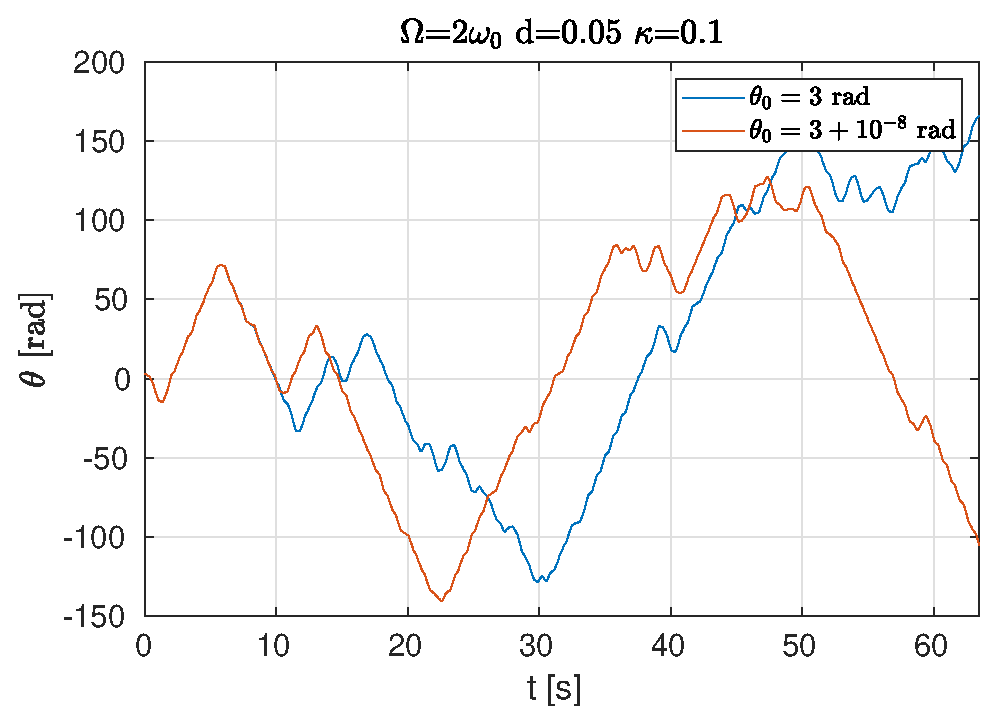
\includegraphics[width=0.91\linewidth,angle=0]{lyapunovThetaInstable}}
\caption{ \label{lyapunovThetaInstable}\em
\textbf{Cas chaotique}, angle du pendule en fonction du temps pour deux angles initiaux très proches et pour $\vt_0=0$. Après une dizaine de secondes, les angles ne sont plus confondus (à l'échelle étudiée) et leur évolution devient très différente.
}
\end{figure}

\begin{figure}[H]
    \centerline{\includegraphics[width=0.9\linewidth,angle=0]{lyapunovOrbiteInstable}}
\caption{ \label{lyapunovOrbiteInstable}\em
Détermination de l'exposant de Lyapunov $\lambda$, qui est la pente de $ln(d(t))$ dans la phase initiale du mouvement, durant laquelle la distance entre les deux orbites (résultant de conditions initiales très proches) grandit exponentiellement.  Conditions initiales : $\t_{0,a}=3\rm{rad}$, $\t_{0,b}=(3+10^{-8})\rm{rad}$, $\vt_{0,a}=\vt_{0,b}=0$
}
\end{figure}
Dans un cas non-chaotique, on peut à nouveau étudier l'évolution de l'angle du pendule pour deux angles initiaux très proches (différence de $10^{-8}\rm{rad}$). On peut voir que la différence entre les deux angles reste très petite avec le temps (Fig.\ref{lyapunovThetaStable} et Fig.\ref{lyapunovThetaStableZoom}). En fait, même leurs orbites dans l'espace des phases restent très similaires (Fig.\ref{lyapunovOrbiteStable}) et ce résultat était prévisible dans un cas non-chaotique : des conditions initiales proches donnent des mouvements similaires. 
\begin{figure}[H]
    \centerline{\includegraphics[width=0.95\linewidth,angle=0]{lyapunovThetaStable}}
\caption{ \label{lyapunovThetaStable}\em
\textbf{Cas non-chaotique}, angle du pendule en fonction du temps pour deux angles initiaux très proches et pour $\vt_0=0$. Les angles sont confondus (à l'échelle étudiée) jusqu'à la fin de la simulation.
}
\end{figure}

\begin{figure}[H]
    \centerline{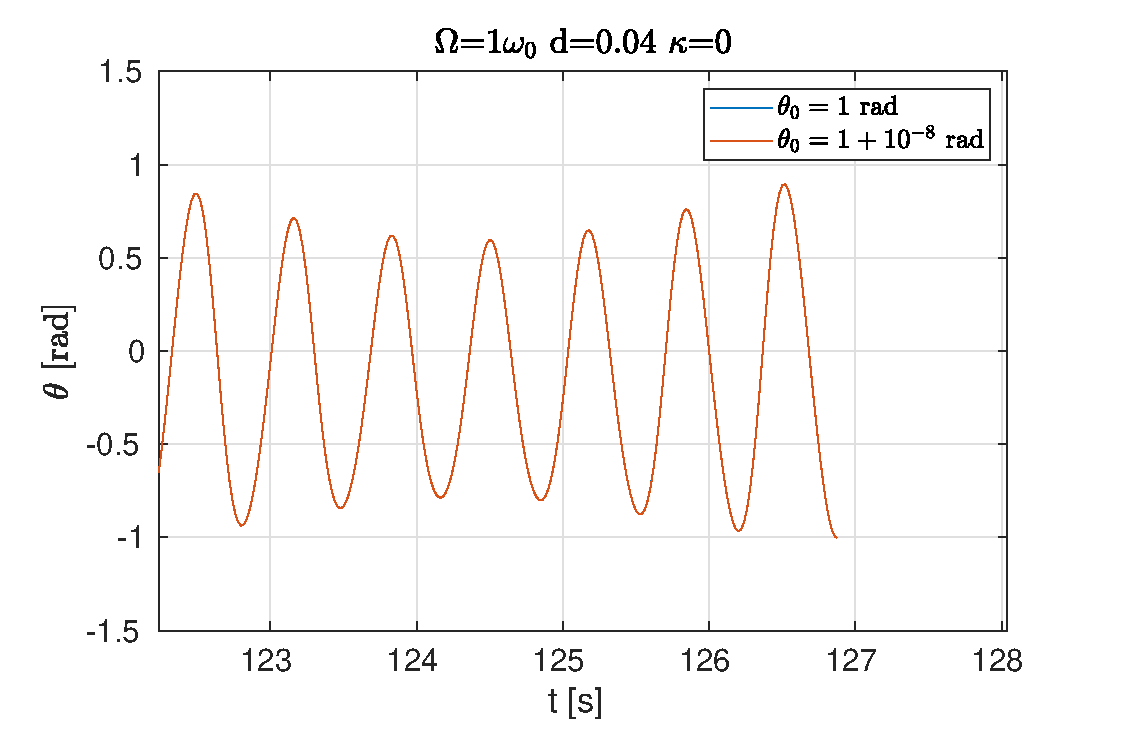
\includegraphics[width=0.95\linewidth,angle=0]{lyapunovThetaStableZoom}}
\caption{ \label{lyapunovThetaStableZoom}\em
Agrandissment de la Fig.\ref{lyapunovThetaStable}.
}
\end{figure}

\begin{figure}[H]
    \centerline{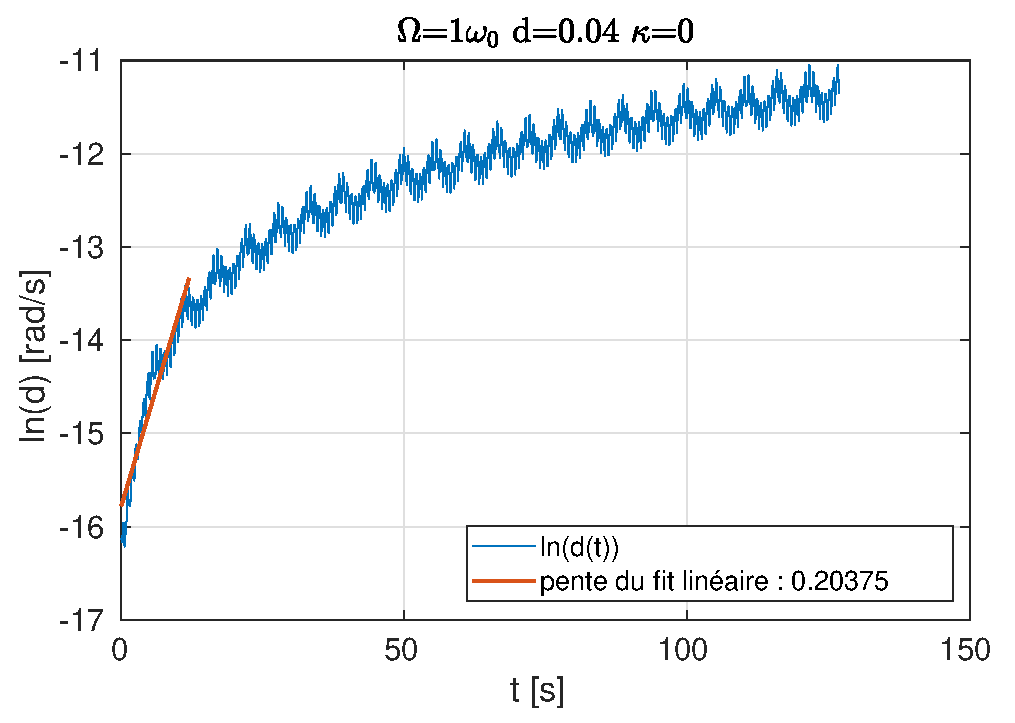
\includegraphics[width=0.95\linewidth,angle=0]{lyapunovOrbiteStable}}
\caption{ \label{lyapunovOrbiteStable}\em
La distance entre les deux orbites restent très faibles : deux conditions initiales très proches donnes des orbites dans l'espace des phases très proches.
}
\end{figure}

%%%%%%%%%%%%%%%%%%%%%%%%%%%%%%%%%%%%%%%%%%%%%%%%%%%%%%%%%%%%%%%%%%%%%%%%%%%%%%%%%%%%%%%%%%%%%%%%%%%%%%%%
\subsection{Section de Poincaré, amorti}
Nous réalisons comme à la section précédente des sections de Poincaré, données par $\{(\t(t_i),\vt(t_i)) : t_i=i2\pi/\Omega \}_{i \in [i_s,i_e]}$, mais cette fois-ci avec un pendule amorti ($\kappa \neq 0$). On peut essayer de jouer avec les conditions initiales et l'amplitude de l'excitation pour essayer de trouver différents attracteurs étranges. 

Par exemple les paramètres $\Omega=2\omega_0$, $d=0.05\rm{m}$ et $\kappa=0.1\rm{kgs^{-2}}$ donnent un attracteur étrange : comme on peut le voir sur la Fig.\ref{attracteur1_1}, deux conditions initiales proches (même vitesse angulaire initiale et différence de $10^{-8}\rm{rad}$ entre les deux angles initiaux) donnent des sections de Poincaré de structure similaire. Cependant en regardant plus en détail, on peut voir sur la Fig.\ref{lyapunovThetaInstableAmorti1} que leurs angles ne concordent plus du tout après $10\rm{s}$. Leurs orbites dans l'espace des phases $(\t,\vt)$ divergent même fortement (Fig.\ref{lyapunovOrbiteInstableAmorti1}).\\
En prenant des conditions initiales assez différentes, on obtient à nouveau des sections de Poincaré à l'allure générale similaire que pour des conditions initiales proches, d'où le nom d'attracteur étrange : toutes kes conditions initiales donnent des sections de Poincaré de structure similaire (avec des zones interdites dans l'espace $(\t,\vt)$), mais des conditions initiales très proches donnent des mouvements divergeant.

\begin{figure}[H]
    \centerline{\includegraphics[width=0.85\linewidth,angle=0]{attracteur1_1}}
\caption{ \label{attracteur1_1}\em
 sections de Poincaré pour deux angles initiaux très proches et pour $\vt_0=0$.
}
\end{figure}
\begin{figure}[H]
    \centerline{\includegraphics[width=0.9\linewidth,angle=0]{lyapunovThetaInstableAmorti1}}
\caption{ \label{lyapunovThetaInstableAmorti1}\em
 Évolution de l'angle du pendule pour deux angles initiaux très proches et pour $\vt_0=0$. Il s'agit bien d'un cas chaotique, les angles divergent après peu de temps.
}
\end{figure}
\begin{figure}[H]
    \centerline{\includegraphics[width=0.85\linewidth,angle=0]{lyapunovOrbiteInstableAmorti1}}
\caption{ \label{lyapunovOrbiteInstableAmorti1}\em
 La distance entre les deux orbites suit bien un comportement exponentielle dans la phase initiale du mouvement. on peut déterminer le coefficient de Lyapunov $\lambda$, donné par la pente de $\ln{(d(t))}$.
}
\end{figure}
\begin{figure}[H]
    \centerline{\includegraphics[width=0.85\linewidth,angle=0]{attracteur1_2}}
\caption{ \label{attracteur1_2}\em
 Deux angles initiaux très différents (et $\vt_0=0$) donnent des sections de Poincaré à la structure similaire : c'est une des signatures des attracteurs étranges.
}
\end{figure}


%%%%%%%%%%%%%%%%%%%%%%%%%%%%%%%%%%%%%%%%%%%%%%%%%%%%%%%%%%%%%%%%%%%%%%%%%%%%%%%%%%%%%%%%%%%%%%%%%%%%%%%%
%%%%%%%%%%%%%%%%%%%%%%%%%%%%%%%%%%%%%%%%%%%%%%%%%%%%%%%%%%%%%%%%%%%%%%%%%%%%%%%%%%%%%%%%%%%%%%%%%%%%%%%%
%%%%%%%%%%%%%%%%%%%%%%%%%%%%%%%%%%%%%%%%%%%%%%%%%%%%%%%%%%%%%%%%%%%%%%%%%%%%%%%%%%%%%%%%%%%%%%%%%%%%%%%%
\newpage \section{Pour aller plus loin ...}
%%%%%%%%%%%%%%%%%%%%%%%%%%%%%%%%%%%%%%%%%%%%%%%%%%%%%%%%%%%%%%%%%%%%%%%%%%%%%%%%%%%%%%%%%%%%%%%%%%%%%%%%
\subsection{Stabilisation à $\t=\pi$}
Le pendule possède deux positions d'équilibre : $\t=0$ et $\t=\pi$. La première est stable alors que la deuxième est instable dans le cas général. Il cependant est possible de stabiliser cette dernière en choisissant judicieusement les paramètres du système. C'est notamment le cas en prenant $\Omega=6\omega_0$, $d=0.03 \rm{m}$, $\vt_0=0$ et $\t_0$ suffisamment proche de $\pi$. On peut différencier le cas amorti et non-amorti. Comme on peut le voir sur Fig.\ref{poincarePI} et Fig.\ref{stabilisationPI}, en prenant $\kappa=0.05\rm{kgs^{-2}}$ (cas amorti), l'angle $\t$ va converger vers $\pi$ et $\vt$ vers $0$ pour des $\t_0$ suffisamment proches de $\pi$. Alors que dans le cas non-amorti (Fig.\ref{poincarePIsansFrot} et Fig.\ref{stabilisationPIsansFrot}), l'angle $\t$, resp. $\vt$, va effectuer de petites oscillations autour de $\pi$, resp. $0$.
\vspace{2cm}
\begin{figure}[H]
    \centerline{\includegraphics[width=0.95\linewidth,angle=0]{poincarePI}}
\caption{ \label{poincarePI}\em
$\t=\pi \pm 0.01 \rm{rad}$, $\vt=0$, $\Omega = 6 \omega_0$, $d=0.03$, $\kappa=0.05$
}
\end{figure}

\begin{figure}[H]
    \centerline{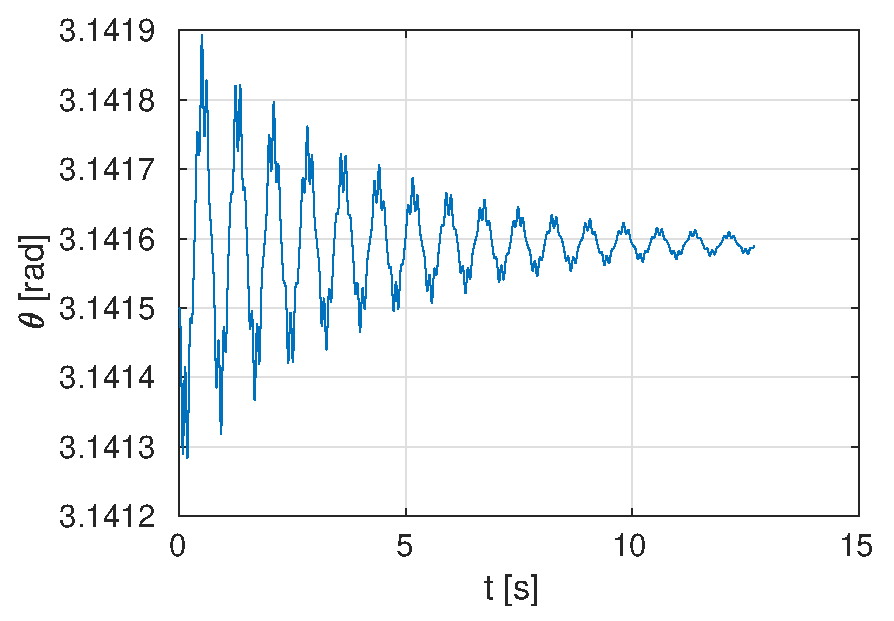
\includegraphics[width=0.6\linewidth,angle=0]{stabilisationPI}}
\caption{ \label{stabilisationPI}\em
$\t=3.1415 \rm{rad}$, $\vt=0$, $\Omega = 6 \omega_0$, $d=0.03$, $\kappa=0.05$
}
\end{figure}
\begin{figure}[H]
    \centerline{\includegraphics[width=0.6\linewidth,angle=0]{poincarePIsansFrot}}
\caption{ \label{poincarePIsansFrot}\em
$\t=\pi-0.02, \pi+0.01 \rm{rad}$, $\vt=0$, $\Omega = 6 \omega_0$, $d=0.03$, $\kappa=0$
}
\end{figure}
\begin{figure}[H]
    \centerline{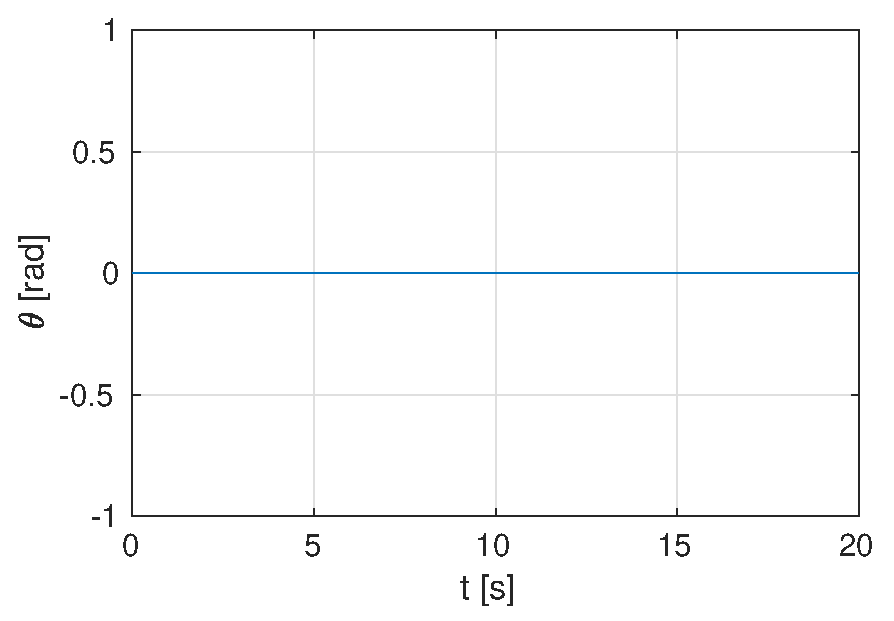
\includegraphics[width=0.6\linewidth,angle=0]{stabilisationPIsansFrot}}
\caption{ \label{stabilisationPIsansFrot}\em
$\t=3.1415 \rm{rad}$, $\vt=0$, $\Omega = 6 \omega_0$, $d=0.03$, $\kappa=0$
}
\end{figure}

%%%%%%%%%%%%%%%%%%%%%%%%%%%%%%%%%%%%%%%%%%%%%%%%%%%%%%%%%%%%%%%%%%%%%%%%%%%%%%%%%%%%%%%%%%%%%%%%%%%%%%%%
\subsection{Galerie d'attracteurs}
\newenvironment{changemargin}[2]{\begin{list}{}{%  
\setlength{\topsep}{0pt}%
\setlength{\leftmargin}{0pt}%
\setlength{\rightmargin}{0pt}%
\setlength{\listparindent}{\parindent}%
\setlength{\itemindent}{\parindent}%
\setlength{\parsep}{0pt plus 1pt}%
\addtolength{\leftmargin}{#1}%
\addtolength{\rightmargin}{#2}%
}\item }{\end{list}}
\begin{changemargin}{-3cm}{-3cm}

\vspace{0.5cm}
\begin{minipage}{0.65\textwidth}
  \centerline{\includegraphics[width=0.91\linewidth,angle=0]{attracteur2}}
\captionof{figure}{Attracteur 1}
\label{Attracteur2}    
\end{minipage}
\begin{minipage}{0.65\textwidth}
    \centerline{\includegraphics[width=0.92\linewidth,angle=0]{attracteur3}}
\captionof{figure}{Attracteur 2}
\label{Attracteur3} 
\end{minipage}

\vspace{0.5cm}
\begin{minipage}{0.65\textwidth}
    \centerline{\includegraphics[width=0.95\linewidth,angle=0]{attracteur3Zoom1}}
\captionof{figure}{Zoom sur l'attracteur 2}
\label{attracteur3Zoom1}   
\end{minipage}
\begin{minipage}{0.65\textwidth}
    \centerline{\includegraphics[width=0.95\linewidth,angle=0]{attracteur3Zoom3}}
    \captionof{figure}{Zoom sur l'attracteur 2}
\label{attracteur3Zoom3}   
\end{minipage}

\vspace{0.5cm}
\begin{minipage}{0.65\textwidth}
  \centerline{\includegraphics[width=0.95\linewidth,angle=0]{attracteur4}}
\captionof{figure}{Attracteur 3}
\label{attracteur4B}    
\end{minipage}
\begin{minipage}{0.65\textwidth}
  \centerline{\includegraphics[width=0.95\linewidth,angle=0]{attracteur4Zoom2}}
\captionof{figure}{Zoom sur l'attracteur 3}
\label{attracteur4Zoom2B}    
\end{minipage}
%%%%


\vspace{3cm}
\begin{minipage}{0.68\textwidth}
  \centerline{\includegraphics[width=0.97\linewidth,angle=0]{attracteur4Zoom3}}
\captionof{figure}{Zoom sur l'attracteur 3}
\label{attracteur4Zoom3B}    
\end{minipage}
\begin{minipage}{0.68\textwidth}
  \centerline{\includegraphics[width=0.97\linewidth,angle=0]{attracteur5}}
\captionof{figure}{Attracteur 4}
\label{attracteur5B}    
\end{minipage}


\vspace{3cm}
\begin{minipage}{0.68\textwidth}
  \centerline{\includegraphics[width=1.00\linewidth,angle=0]{attracteur5Zoom1}}
\captionof{figure}{Zoom sur l'attracteur 4}
\label{attracteur5Zoom1B}    
\end{minipage}
\begin{minipage}{0.68\textwidth}
  \centerline{\includegraphics[width=1.00\linewidth,angle=0]{attracteur5Zoom2}}
\captionof{figure}{Zoom sur l'attracteur 4}
\label{attracteur5Zoom2B}    
\end{minipage}

%%%%%%%%%%%%%%%%%%%%%%%%%%%%%%%%%%
%\begin{figure}[H]
%    \centerline{\includegraphics[width=0.95\linewidth,angle=0]{attracteur4}}
%\caption{ \label{attracteur4}\em
%Attracteur 3
%}
%\end{figure}


%\begin{figure}[H]
%    \centerline{\includegraphics[width=0.95\linewidth,angle=0]{attracteur4Zoom2}}
%\caption{ \label{attracteur4Zoom2}\em

%}
%\end{figure}


%\begin{figure}[H]
%    \centerline{\includegraphics[width=0.95\linewidth,angle=0]{attracteur4Zoom3}}
%\caption{ \label{attracteur4Zoom3}\em
%Zoom sur l'attracteur 3
%}
%\end{figure}


%\begin{figure}[H]
    %\centerline{\includegraphics[width=0.95\linewidth,angle=0]{attrac%teur5}}
%    \caption{ \label{attracteur5}\em
%Attracteur 4
%}
%\end{figure}


%\begin{figure}[H]
 %   \centerline{\includegraphics[width=0.95\linewidth,angle=0]{attracteur5Zoom1}}
%\caption{ \label{attracteur5Zoom1}\em
%Zoom sur l'attracteur 4
%}
%\end{figure}


%\begin{figure}[H]
 %   \centerline{\includegraphics[width=0.95\linewidth,angle=0]{attracteur5Zoom2}}
%\caption{ \label{attracteur5Zoom2}\em
%Zoom sur l'attracteur 4
%}
%\end{figure}
\end{changemargin}


%%%%%%%%%%%%%%%%%%%%%%%%%%%%%%%%%%%%%%%%%%%%%%%%%%%%%%%%%%%%%%%%%%%%%%%%%%%%%%%%%%%%%%%%%%%%%%%%%%%%%%%%
%%%%%%%%%%%%%%%%%%%%%%%%%%%%%%%%%%%%%%%%%%%%%%%%%%%%%%%%%%%%%%%%%%%%%%%%%%%%%%%%%%%%%%%%%%%%%%%%%%%%%%%%
%%%%%%%%%%%%%%%%%%%%%%%%%%%%%%%%%%%%%%%%%%%%%%%%%%%%%%%%%%%%%%%%%%%%%%%%%%%%%%%%%%%%%%%%%%%%%%%%%%%%%%%%
\newpage \section{Conclusion}
Cette expérience nous a appris beaucoup de chose sur les trajectoires de pendule dans le cas harmonique et non-harmonique. On a pu faire des simulations sur des oscillations de petites ou grandes amplitudes, avec ou sans amortissement et avec ou sans excitation. Certain de ces cas possèdent une solution analytique nous permettant ainsi d'effectuer une comparaison et de valider les résultats obtenus par nos méthodes méthodes numériques. Ces méthodes étant ainsi éprouvés, nous avons pu les utiliser pour simuler des trajectoires dans des cas plus complexes, où il n'était pas possible d'obtenir la solution analytiquement, démontrant ainsi l'utilité de ces méthodes numériques. Des cas spécifiques ont pu être étudiés tels que la résonance et la résonance paramétrique. Nous avons également pu étudier des trajectoires de type chaotique et en tirer des conclusions, comme par exemple que malgré leurs imprévisibilités, ces mouvement peuvent posséder une certaine structure et parfois converger vers certains points.




%%%%%%%%%%%%%%%%%%%%%%%%%%%%%%%%%%%%%%%%%%%%%%%%%%%%%%%%%%%%%%%%%%%%%%%%%%%%%%%%%%%%%%%%%%%%%%%%%%%%%%%%
%%%%%%%%%%%%%%%%%%%%%%%%%%%%%%%%%%%%%%%%%%%%%%%%%%%%%%%%%%%%%%%%%%%%%%%%%%%%%%%%%%%%%%%%%%%%%%%%%%%%%%%%
%%%%%%%%%%%%%%%%%%%%%%%%%%%%%%%%%%%%%%%%%%%%%%%%%%%%%%%%%%%%%%%%%%%%%%%%%%%%%%%%%%%%%%%%%%%%%%%%%%%%%%%%
\begin{thebibliography}{99}
\bibitem{donneeEX2} 
Données de l'exercice 2. Laurent Villard, EPFL, 2018.
\bibitem{notesDeCours}
Physique numérique I/II, notes de cours. Laurent Villard, EPFL, 2018.
\bibitem{stubbe}
Analyse II, note de cours, pp.120-121. Joachim Stubbe, EPFL, 2018.
 \end{thebibliography}
\end{document}

